\section{Resultater}

\subsection{M�linger i romtemperatur}

Figur \ref{fig:erbium_gammel} og \ref{fig:erbium_ny} viser Erbium referansepr�ve ved 300K, pumpet med 532nm laser, med grating lik 300.

%Erbium_gammel.eps
%Erbium_ny.eps

\begin{figure}[H]
\centering
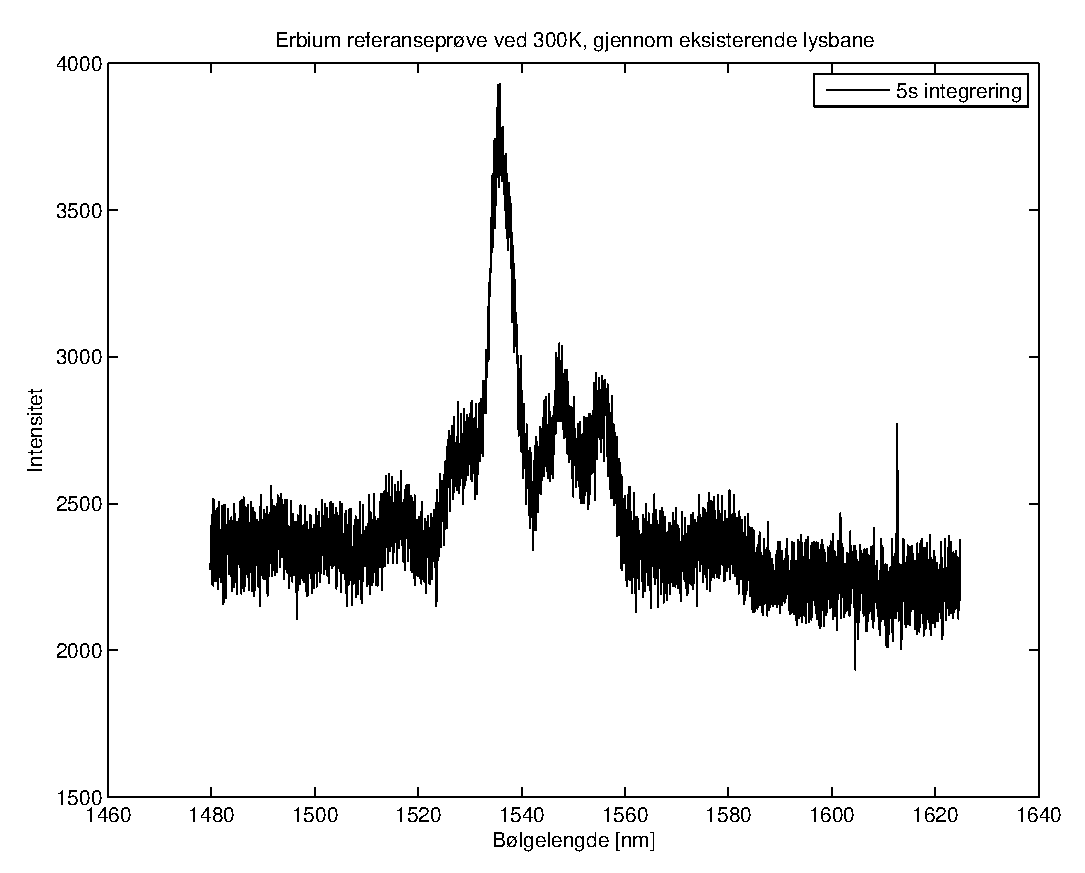
\includegraphics[scale=0.5]{Erbium_gammel.eps}
\caption{Eksitert lys sendt gjennom eksisterende laboppsett, med grating rundt 1550nm}%
\label{fig:erbium_gammel}%
\end{figure}

\begin{figure}[H]
\centering
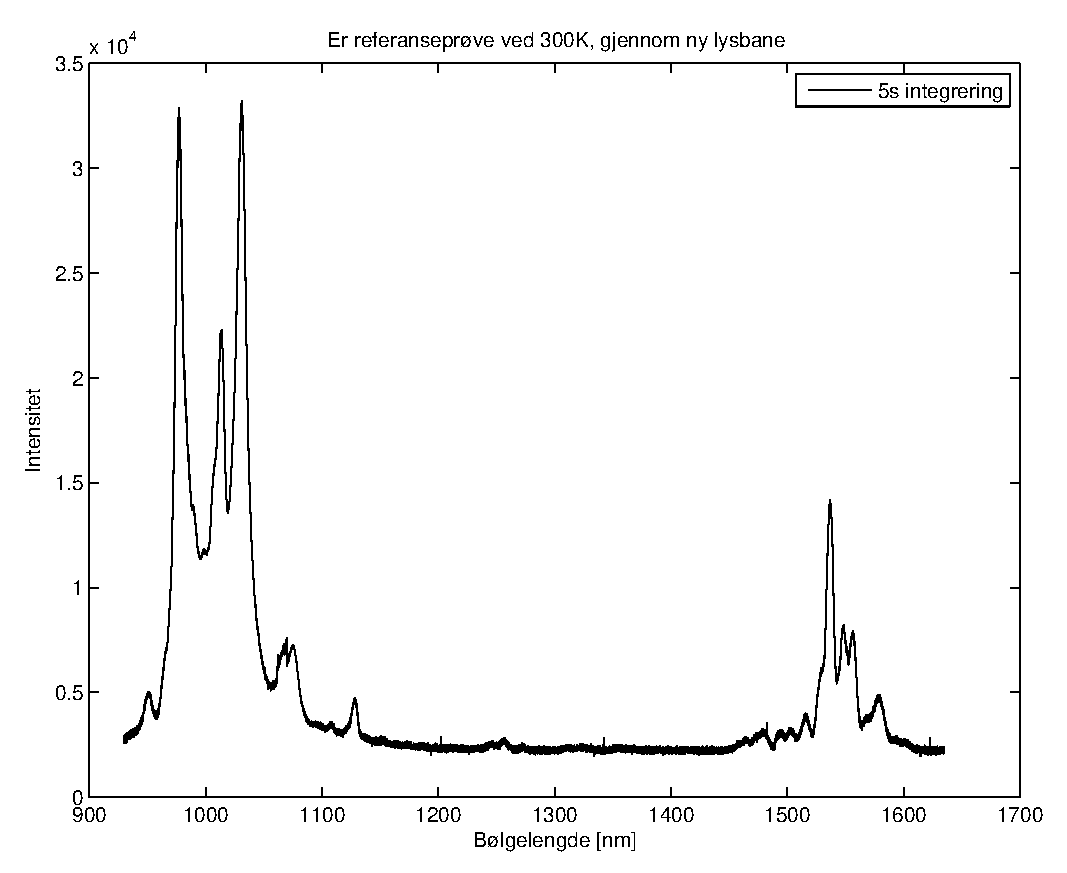
\includegraphics[scale=0.5]{Erbium_ny.eps}
\caption{Eksitert lys sendt gjennom nye komponenter}%
\label{fig:erbium_ny}%
\end{figure}

%Polert_300K.eps
%Upolert_300K.eps

Figur \ref{fig:polert_sample} og \ref{fig:upolert} er m�linger gjort ved 300K, pumpelys lik 532nm, og grating lik 300. Den upolerte pr�ven er samme som i figur \ref{fig:cryolabtap}. Den andre pr�ven i figur \ref{fig:upolert_sample} er lik p� alle m�ter, bortsett fra at den er polert p� overflaten.

\begin{figure}[H]%
\centering
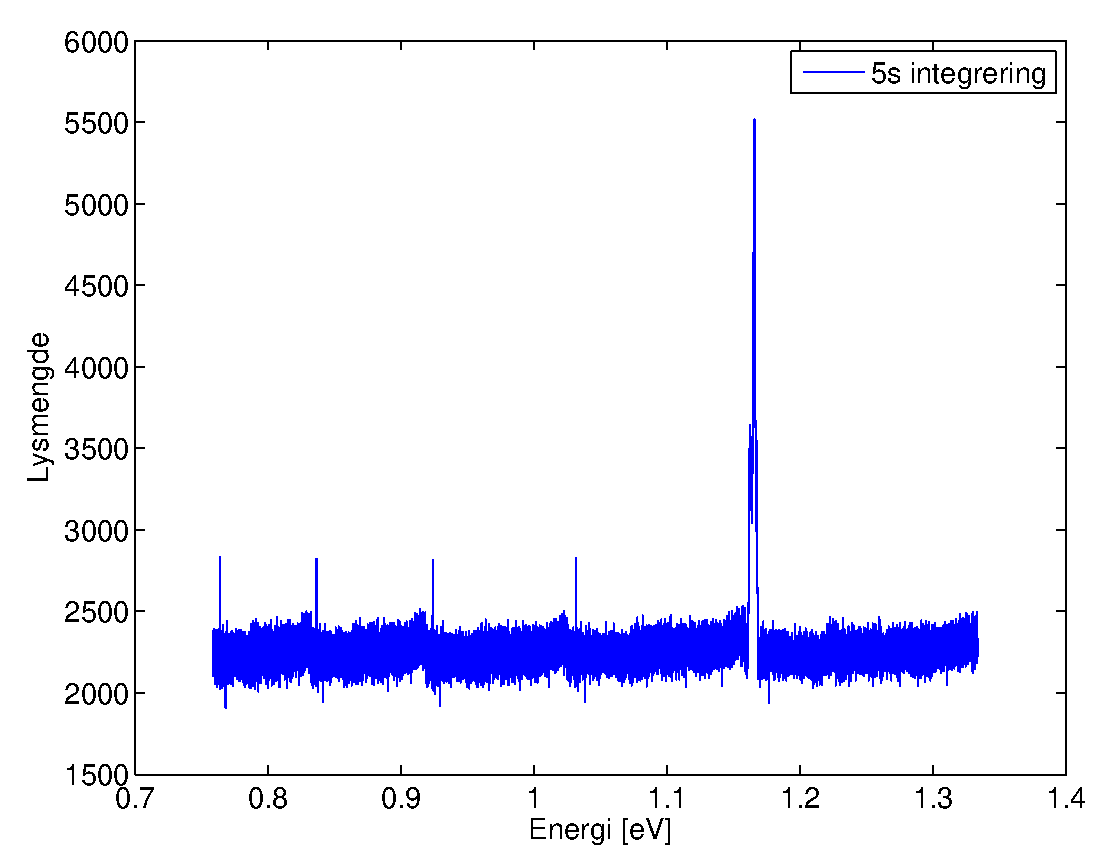
\includegraphics[scale=0.5]{Polert_300K.eps}
\caption{Polert multikrystallinsk silisium}%
\label{fig:upolert}%
\end{figure}

\begin{figure}[H]%
\centering
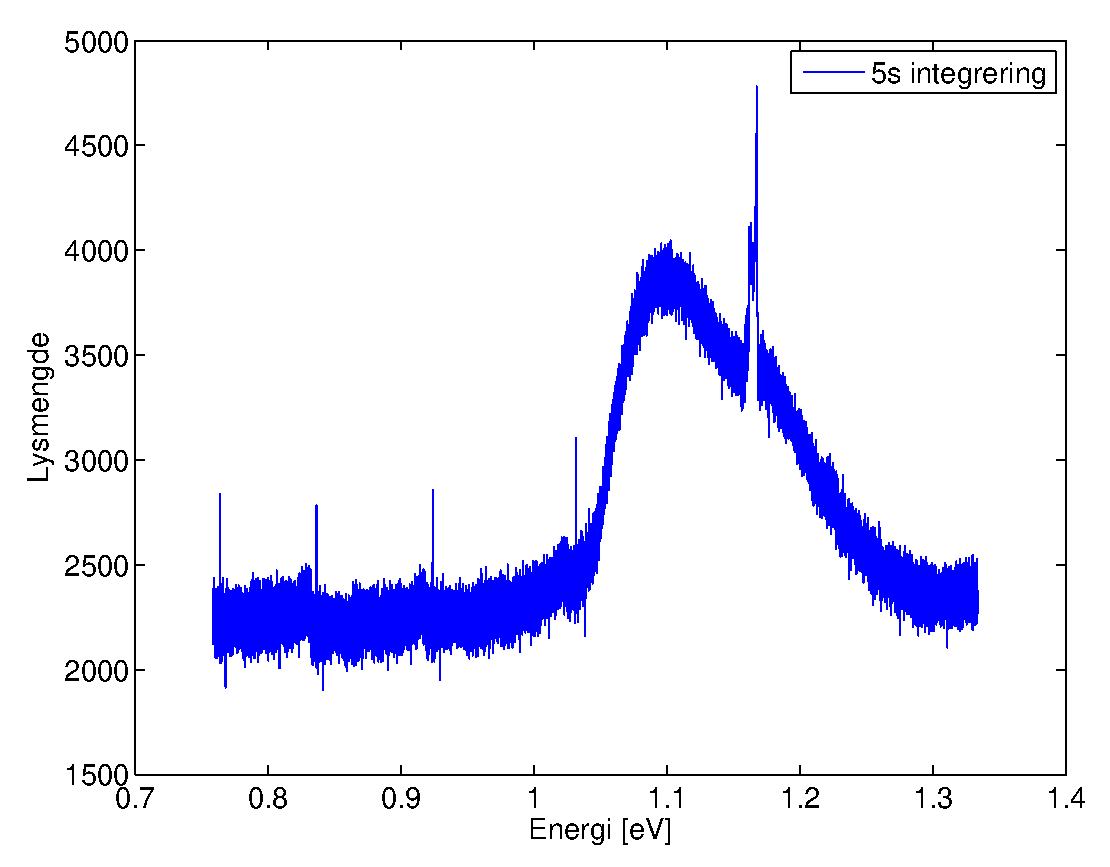
\includegraphics[scale=0.5]{Upolert_300K.eps}
\caption{Upolert multikrystallinsk silisium}%
\label{fig:polert}%
\end{figure}

\subsection{M�linger ved lavtemperatur}




%Posisjonsavhengighet.eps
%Sample_4.eps
%Sample_4_1.eps
%Sample_4_2_1.eps
%Sample_4_2_2.eps
%Sample_4_SPOT_1_BAD.eps
%Sample_4_SPOT_2_GOOD.eps



